\section{Vision Language Models}
Vision language models (VLMs) are artificial intelligence (AI) models that combine both computer vision (CV) and natural language processing (NLP) techniques and capabilities, these models are designed to jointly understand and reason visual and textual information simultaneously \cite{bolcato_vlm_2024} \cite{ibm_vlm_2024}. Among the most well-known models which will be covered when corresponded, models such as GPT-5, Gemini and LLaVA could be highlighted.

In comparison to the traditional models that process data modalities independently, VLMs have been shaped to align textual and visual data, enabling to reason complex scenes and natural language instructions.

\subsection{History of VLMs}
VLMs are the result of the evolution to earlier image captioning systems, systems which were designed primarily to take isolated images and produce descriptions. However, this systems just received the image as input, not an image-text pair input as the vision language models do now \cite{wiki:Vision-language_model}.

\subsubsection{Earliest models}
The early image captioning systems from around year 2010 used the \textit{encoder-decoder} architecture, which will be described later on. These models would encode the patched images and vectorize them into feature vectors, which were then fed to the decoder part in order to generate the associated output description. When it comes to the strategies implemented by this earliest models include combination of handcrafted \textit{visual features} to encode the image patches and \textit{n-gram} templates to generate the description. 

Those visual features can refer to any visual property like points, edges or even objects in the image. % explain a little bit more?

On the other hand, n-grams are statistical language models that calculate the probability of the next word in a sequence from a fixed size window of previous words. Depending on the number of previous words considered, we can get bigram models if just one previous word is considered, if it's two is a trigram model, ... up to \textit{n} - 1 considered as \textit{n-gram} models and finally an unigram if no previous context is considered. 

The general approximation for a sequence of words $w_1, \dots, w_m$ is:
\[
P(w_1, \dots, w_m) \approx \prod_{i=1}^{m} P(w_i \mid w_{i-(n-1)}, \dots, w_{i-1})
\]

\begin{itemize}
	\item Unigram Model ($n=1$): No context, independent probabilities.
	\[
	P(w_1, \dots, w_m) \approx \prod_{i=1}^{m} P(w_i)
	\]
	
	\item Bigram Model ($n=2$): Depends on the single previous word.
	\[
	P(w_1, \dots, w_m) \approx \prod_{i=1}^{m} P(w_i \mid w_{i-1})
	\]
	
	\item Trigram Model ($n=3$): Depends on the two previous words.
	\[
	P(w_1, \dots, w_m) \approx \prod_{i=1}^{m} P(w_i \mid w_{i-2}, w_{i-1})
	\]
\end{itemize}

\subsubsection{Deep learning based models}
When the deep learning neural networks arose and became dominant near year 2015, newer models and strategies also emerged. Convolutional neural networks (CNNs) started to being used for image encoding and recurrent neural networks (RNNs) to generate the captions.

% Explain CNNs and RNNs?

However by 2018, the transformer architecture replaced the sequential recurrent neural networks in the role as decoders. In parallel, the network parameter training started relying on image-text pair datasets, and the scope of VLMs widened until reaching other tasks. Among those tasks, \textit{phrase grounding} could be mentioned. Task involving both natural language processing and computer vision where words or phrases within a sentence are associated to corresponding patches in an image \cite{timothy2024phrasegrounding}. Consists of identifying the spatial location within an image that aligns with the meaning of a given phrase, enabling models to map visual and textual data. 

\begin{figure}[H]
	\centering
	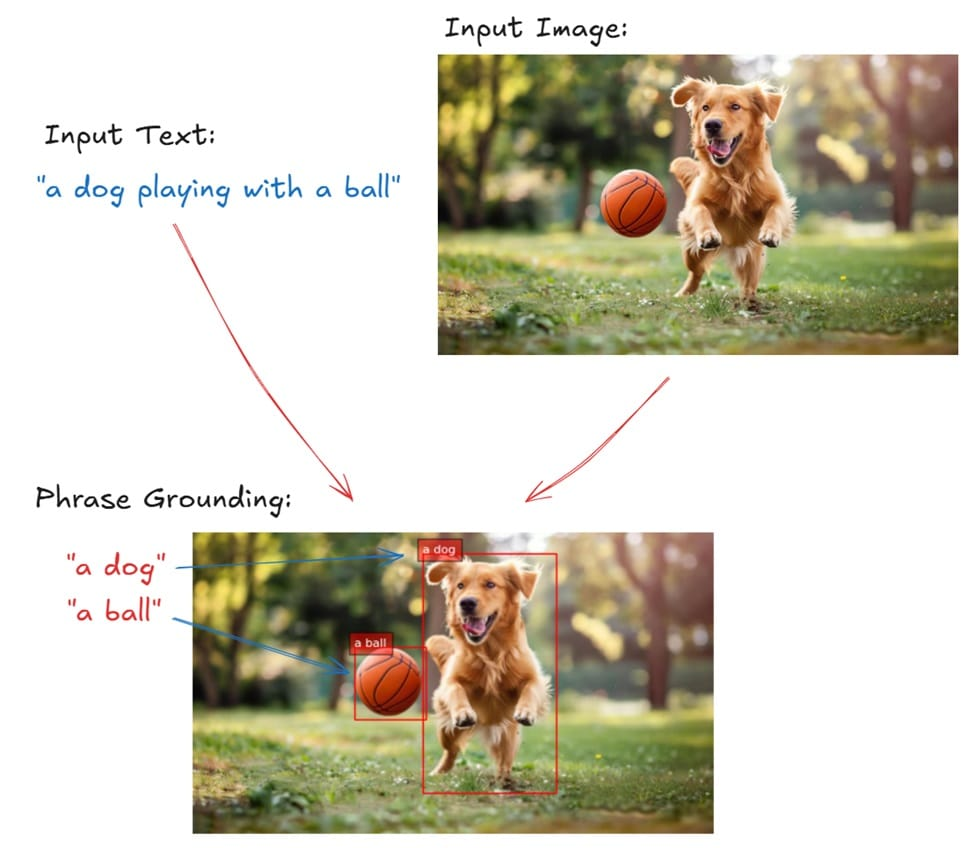
\includegraphics[width=0.5\textwidth]{imgs/phrase_grounding.jpg}
	\caption{Graphical example of phrase grounding}
	\label{fig:phrase_grounding_example}
\end{figure}

Another task which still remains as perhaps the most relevant one is \textit{visual question answering} (VQA). Specific task where the model is provided with an image and a specific related question, and it must generate an accurate response to it based on the visual content. Being its core pillars the object detection duty for identifying the objects in the image, then scene understanding to map the relations between objects and then finally text comprehension for embedded text interpretation within an image \cite{gravio2025vlmvqa}. 

\subsubsection{2021 - Release of CLIP}
In the year 2021, OpenAI launched the approach that would totally revolution the evolution of vision language models, they released the method of \textit{contrastive language-image pretraining} also known as \textit{CLIP}. Technique for training an image-text pair into neural network models, having an exclusive neural network for image and text understanding purposes, adopting a contrastive objective. 

When it comes to the algorithm itself, each neural network receives the input in the corresponding format and returns a single semantic/visual representative vector \cite{wiki:clip}. The objective to maximize by both models is the best alignment between both output vectors in the shared vector space, mapping the similar text-image pairs as close as possible while putting apart the most dissimilar ones. The training relies on a huge dataset with image-text pairs as and the two output vectors are considered similar depending on the \textit{dot product} value. 

% dot prodcut formula
\begin{equation}
	s_{i,j} = \mathbf{v}_i \cdot \mathbf{w}_j = \sum_{k=1}^{d} v_{i,k} w_{j,k}
\end{equation}
where $\mathbf{v}_i$ and $\mathbf{w}_j$ represent the embedding vectors generated by the text and image encoders respectively, and $d$ denotes the dimensionality of the vector space. The loss function used is the multi-class N-pair loss, which is a symmetric \textit{cross-entropy loss} over the similarity scores. The function fosters the dot product between the matching image and text vectors to be as high as possible, while discouraging high dot products between mismatching pairs. 

% loss function formula
\begin{equation}
	\mathcal{L} = -\frac{1}{N} \sum_{i} \ln \frac{e^{v_i \cdot w_i / \tau}}{\sum_{j} e^{v_i \cdot w_j / \tau}} - \frac{1}{N} \sum_{j} \ln \frac{e^{v_j \cdot w_j / \tau}}{\sum_{i} e^{v_i \cdot w_j / \tau}}
\end{equation}
being parameter \textit{T} the temperature parameter (\textit{T}>0) which is parametrized and learned during the training. Other loss functions are possible, such as the \textit{Sigmoid CLIP} function.

Once gone over the algorithm's properties, let's dive deep into the architecture:

\begin{itemize}
	\item Image model: when it comes to the image encoder used in most of the CLIP versions, they all usually are some kind of \textit{vision transformers} (ViT). Vision transformers often vary on the patch size, being that size the \textit{n}x\textit{n} dimensions of the patch the image was divided into. Alternatively, \textit{convolutional neural networks} (CNNs) can be used as well (such as \textit{ResNet}), the essential thing is to ensure the sizes of the image and text model output vectors are the same size. 
	
	\item Text model: the text encoding models are usually \textit{transformers}. Even if it is heavily inspired on the transformers report published by OpenAI \cite{radford2021learningtransferablevisualmodels} and shares similarities with the \textit{GPT} architecture (decoder-only), the text model serves as a text encoder. Furthermore, its functionality is inspired by encoder only models such as \textit{BERT}, while sharing the dimensionality and number of parameters with decoder-only models as mentioned before. 
\end{itemize}

After going over the properties of both encoders that make the whole CLIP model, I will detail the model's workflow inspired on the image below \ref{fig:clip_architecture}. 

\begin{enumerate}
	\item The image of the image-text pair input is first splitted into smaller sized images named patches and then	fed into the vision encoder, which as mentioned earlier, can be any kind of architecture such as a vision transformer (ViT) or convolutional neural network (CNN). The output of the vision encoder will in fact be a vector representation of all the features that have been captured: shapes, texture, colors, objects, spacial relations, ... etc. 
	
	\item Now it's time the model turns those embeddings into real semantic representations, nevertheless, the model still does not know how to label concepts directly. So the model must know combine the embeddings obtained in the image model with the ones from the text model output, aligning them into a shared vector space establishing the real relations and links between the pairs. This bridging mechanism between the image and text pair is where the CLIP model's magic really shines. Although CLIP uses a contrastive allignment strategy in order to put correct pairs closer and dissimilar pairs further in the vector space, there are other models such as \textit{LlaVa} use other tools such as projection layers, where a small network transforms embeddings into LLM token space.
	
	\item Once the image is alligned to the text, that pair is passed to a large language model and then that same LLM takes the combined embeddings and creates meaningful text. 
	
	\item Finally, those LLM outputs are transformed into descriptions or answers depending on the task: classification as in the referenced schema image or other objectives such as visual question answering. 
\end{enumerate}

% image of the CLIP architecture[H], dataset, preprocessing and other things later on.
\begin{figure}[H]
	\centering
	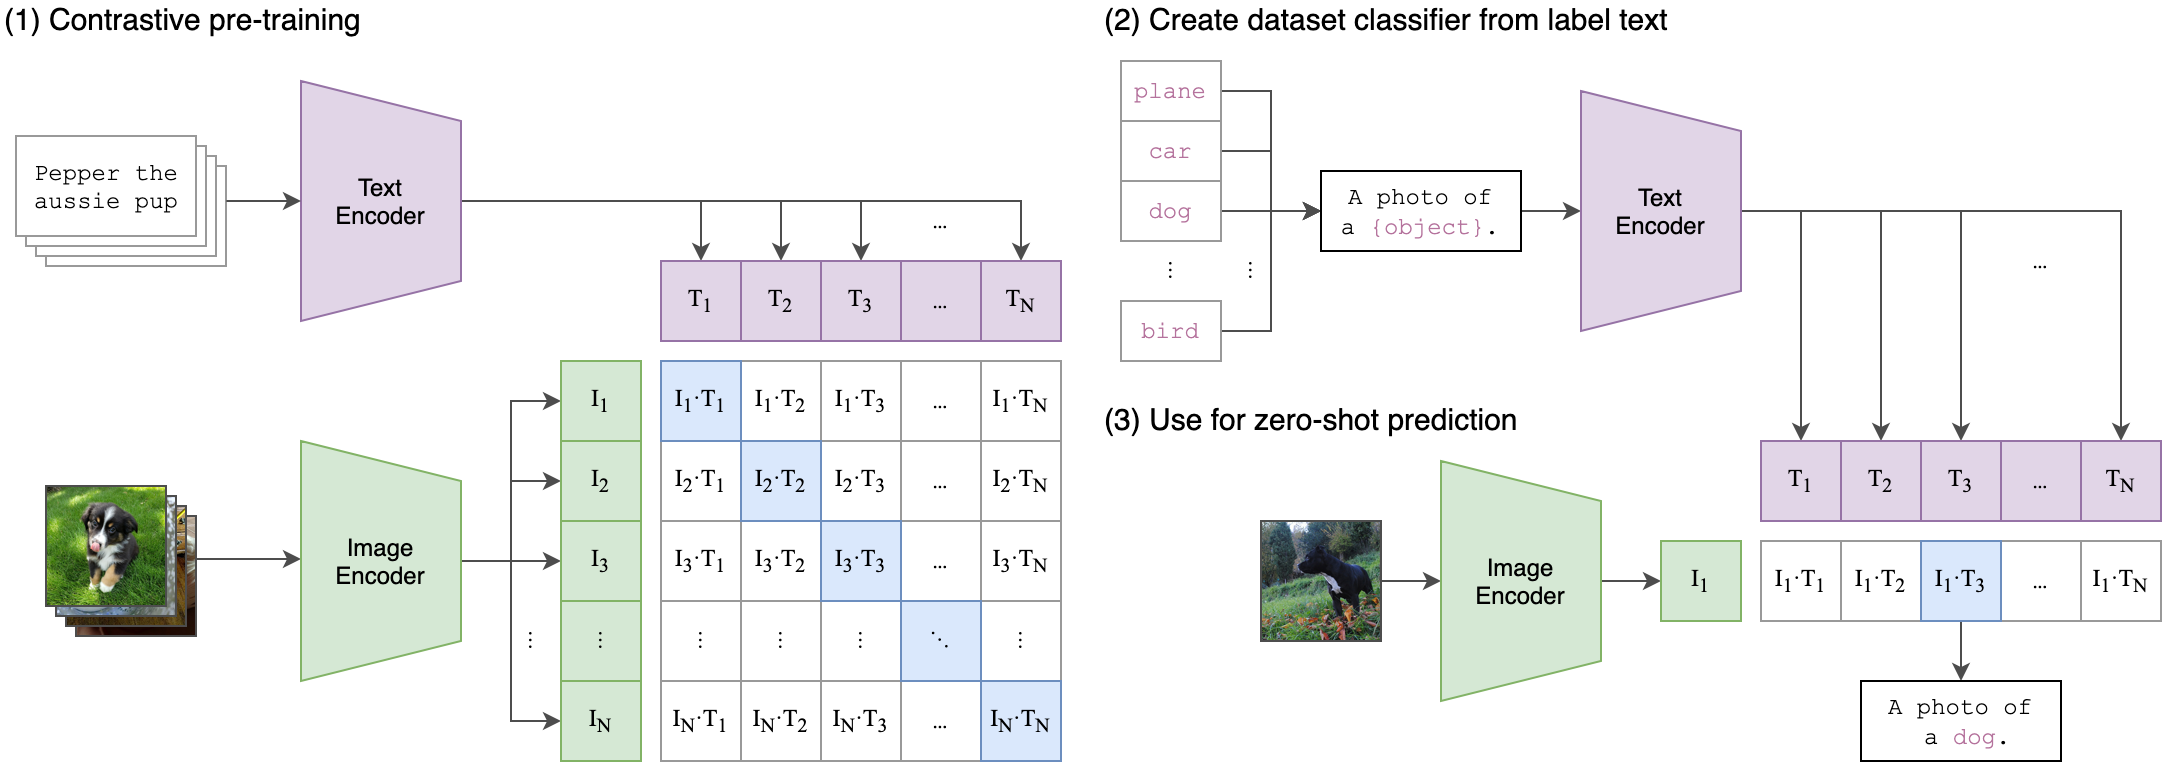
\includegraphics[width=0.8\textwidth]{imgs/CLIP.png}
	\caption{CLIP workflow}
	\label{fig:clip_architecture}
\end{figure}

The reason why these models work so well is because of the millions of image-text pair instances used for training and due to the model's ability to learn and deal with statistical spatial correlations that are shown both in the images and texts.

The dataset the model was trained on is a \textit{WebImageText} (WIT) containing more than 400 million pair instances scraped from the internet, almost half a million text queries and more than 20,000 image-text pairs as query. All of those queries were generated by the most frequent words of the english Wikipedia and then extended using bigrams. The dataset remains private and has never been released. 

Last but not least, images are preprocessed by dividing them into the RGB (reed, green and blue) channels and normalizing the values so they fall between range 0 to 1. Finally those values are merged with the mean and standard deviation of the images from the training dataset. In case the input image does not have the desired resolution (224x224 usually) the image is scaled by \textit{bicubic interpolation} \cite{wiki:bicubic_interpolation} to the shorter sides is the same as the native resolution, and then the central square of the image is cropped out. 

\subsubsection{Models released in the last years}
Since 2022 plenty of new VLM architectures have been published based on similar design and architectures, models such as \textit{Flamingo, LLaVA, InstructBLIP, ...} could be mentioned. All of these models used a separately trained CLIP-like image encoder standard LLMs for text encoding. However, the release of \textit{GPT-4V} in 2023 marked the emergence of commercial implications, followed by the integration of VLMs into the most powerful models such as \textit{Gemini, Copilot and Claude 3 Opus}. These newer applications contained a substantially larger number of parameters, were based on training on larger datasets and were powered by greater computational power. 

\subsection{Elements of a VLMs}
Inspired in other previous model architectures, vision language models consisted on two main components: the \textit{language encoder} and the \textit{visual encoder}. Compared to other \textit{seq2seq} architectures like encoder-only, decoder-only or encoder-decoder, VLMs consist on 2 encoders, one for each data modality encoding task.

\subsubsection{Transformers}

Before going in detail of the components, I will go over the basic architecture most of the VLMs are based on: \textit{transformers}.

\begin{enumerate}
	\item The encoders transform the input sequence into numerical representations called \textit{embeddings} which capture all the semantic and positional meaning of the tokens belonging to the input.
	
	\item Then they use a mechanism called \textit{self-attention} which allows the encoder to focus on the most relevant tokens of the sequence independent of their position.
	
	\item Finally the decoders of the transformers take both the output of the self-attention mechanism and the encoder generated embeddings to generate the most statistically likely output sequence.
\end{enumerate}

\subsubsection{Language encoder} 
This first encoder captures the semantic relations and meanings between the words in the textual prompt given and turns them into \textit{text embeddings} to be processed, carrying the same encoding process seen in the majority of architectures. 

\subsubsection{Vision encoder}
The second encoder extracts the visual properties and patterns from the visual data of the prompt and transforms them into embeddings too. Compared to earlier VLMs which used \textit{convolutional neural networks} (CNNs) for feature extraction such as the colors, shapes and textures from the input, modern ones employ an architecture called \textit{visual transformer} (ViT).

\subsubsection{Visual transformer (ViT)}
Visual transformers process images into smaller patches and treats them as sequences, implementing also the self-attention mechanism across the patches to create a transformer-based representation of the input message.

% geroko
\begin{figure}[H]
	\centering
	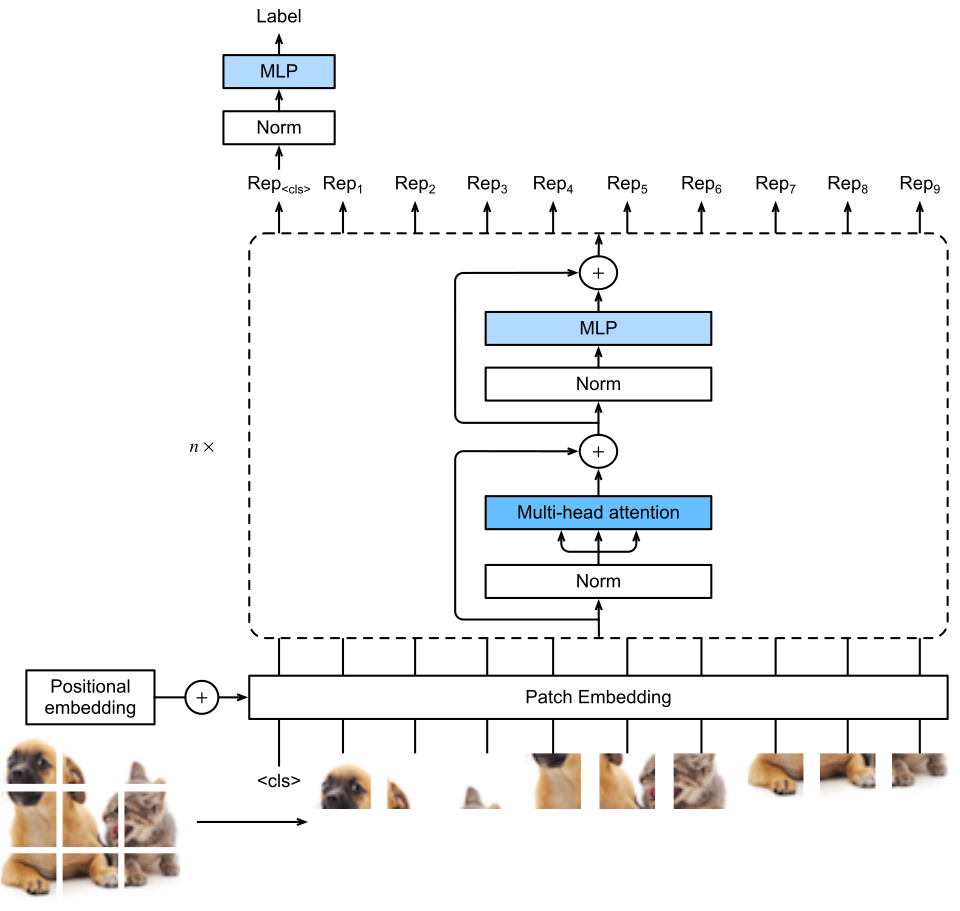
\includegraphics[width=0.7\textwidth]{imgs/Vision_Transformer.png}
	\caption{Vision transformer architecture}
	\label{fig:vit_architecture}
\end{figure}

\section{Reinforcement Learning}

\section{Multi-agent systems}

\section{State of the Art}

\subsection{VLMs evolution}

\subsection{Current models}

\subsection{Benchmarks}

\subsection{VLMs in robotics}

\subsection{Frameworks}